\documentclass[journal]{IEEEtran}
\usepackage[a5paper, margin=10mm, onecolumn]{geometry}
%\usepackage{lmodern} % Ensure lmodern is loaded for pdflatex
\usepackage{tfrupee} % Include tfrupee package

\setlength{\headheight}{1cm} % Set the height of the header box
\setlength{\headsep}{0mm}     % Set the distance between the header box and the top of the text

\usepackage{gvv-book}
\usepackage{gvv}
\usepackage{cite}
\usepackage{amsmath,amssymb,amsfonts,amsthm}
\usepackage{algorithmic}
\usepackage{graphicx}
\usepackage{textcomp}
\usepackage{xcolor}
\usepackage{txfonts}
\usepackage{listings}
\usepackage{enumitem}
\usepackage{mathtools}
\usepackage{gensymb}
\usepackage{comment}
\usepackage[breaklinks=true]{hyperref}
\usepackage{tkz-euclide} 
\usepackage{listings}
% \usepackage{gvv}                                        
\def\inputGnumericTable{}                                 
\usepackage[latin1]{inputenc}                                
\usepackage{color}                                            
\usepackage{array}                                            
\usepackage{longtable}                                       
\usepackage{calc}                                             
\usepackage{multirow}                                         
\usepackage{hhline}                                           
\usepackage{ifthen}                                           
\usepackage{lscape}
\begin{document}

\bibliographystyle{IEEEtran}
\vspace{3cm}

\title{10.3.5.4.4}
\author{EE24BTECH11017 - D.Karthik}
 \maketitle
% \newpage
% \bigskip
{\let\newpage\relax\maketitle}

\renewcommand{\thefigure}{\theenumi}
\renewcommand{\thetable}{\theenumi}
\setlength{\intextsep}{10pt} % Space between text and floats


\numberwithin{equation}{enumi}
\numberwithin{figure}{enumi}
\renewcommand{\thetable}{\theenumi}
\textbf{Problem Statement :}
 Places A and B are 100 km apart on a highway. One car starts from A and another
from B at the same time. If the cars travel in the same direction at different speeds,
they meet in 5 hours. If they travel towards each other, they meet in 1 hour. What
are the speeds of the two cars?
\section*{Solution}
Let:
\begin{itemize}
    \item The speed of the car starting from A be \( x \) km/h.
    \item The speed of the car starting from B be \( y \) km/h.
\end{itemize}

\subsection*{Case 1: Cars Traveling in the Same Direction}
- The relative speed is \( (x - y) \) km/h.
- They meet after 5 hours, so the distance traveled by their relative speed is:
  \[
  5(x - y) = 100
  \]
  \[
  x - y = 20 \quad \text{(Equation 1)}
  \]

\subsection*{Case 2: Cars Traveling Towards Each Other}
- The relative speed is \( (x + y) \) km/h.
- They meet after 1 hour, so the total distance covered is:
  \[
  1(x + y) = 100
  \]
  \[
  x + y = 100 \quad \text{(Equation 2)}
  \]

\subsection*{Solving the Equations}
We now solve the system:
\[
x - y = 20
\]
\[
x + y = 100
\]

Adding both equations:
\[
(x - y) + (x + y) = 20 + 100
\]
\[
2x = 120
\]
\[
x = 60
\]

Substituting \( x = 60 \) into Equation 2:
\[
60 + y = 100
\]
\[
y = 40
\]

\section*{Conclusion}
\begin{itemize}
    \item The speed of the car starting from A is \textbf{60 km/h}.
    \item The speed of the car starting from B is \textbf{40 km/h}.
\end{itemize}


\textbf{Given System of Equations}
\begin{align}
    x - y &= 20 \label{eq1}\\
    x + y &= 100 \label{eq2}
\end{align}

\subsection{Step 1: Matrix Representation}
Rewriting the system in matrix form:

\begin{equation}
    \begin{bmatrix} 
        1 & -1 \\ 
        1 & 1 
    \end{bmatrix}
    \begin{bmatrix} 
        x \\ y 
    \end{bmatrix} =
    \begin{bmatrix} 
        20 \\ 100 
    \end{bmatrix}
\end{equation}

Define:

\begin{align}
    A &= \begin{bmatrix} 1 & -1 \\ 1 & 1 \end{bmatrix}, \quad
    X = \begin{bmatrix} x \\ y \end{bmatrix}, \quad
    B = \begin{bmatrix} 20 \\ 100 \end{bmatrix}
\end{align}

\subsection{Step 2: LU Decomposition}
We express \( A \) as:

\begin{equation}
    A = LU
\end{equation}

where \( L \) is a **lower triangular matrix**, and \( U \) is an **upper triangular matrix**:

\begin{equation}
    L = \begin{bmatrix} 1 & 0 \\ l_{21} & 1 \end{bmatrix}, \quad
    U = \begin{bmatrix} u_{11} & u_{12} \\ 0 & u_{22} \end{bmatrix}
\end{equation}

Expanding:

\begin{equation}
    \begin{bmatrix} 1 & 0 \\ l_{21} & 1 \end{bmatrix}
    \begin{bmatrix} u_{11} & u_{12} \\ 0 & u_{22} \end{bmatrix}
    =
    \begin{bmatrix} 1 & -1 \\ 1 & 1 \end{bmatrix}
\end{equation}

By comparing entries:

\begin{align}
    u_{11} &= 1, \quad u_{12} = -1 \\
    l_{21} \cdot u_{11} &= 1 \Rightarrow l_{21} = 1 \\
    l_{21} \cdot u_{12} + u_{22} &= 1 \Rightarrow (1)(-1) + u_{22} = 1 \Rightarrow u_{22} = 2
\end{align}

Thus:

\begin{align}
    L &= \begin{bmatrix} 1 & 0 \\ 1 & 1 \end{bmatrix}, \quad
    U = \begin{bmatrix} 1 & -1 \\ 0 & 2 \end{bmatrix}
\end{align}

\subsection{Step 3: Solve \( LY = B \) (Forward Substitution)}
We solve:

\begin{equation}
    L Y = B
\end{equation}

where \( Y = \begin{bmatrix} y_1 \\ y_2 \end{bmatrix} \) is an intermediate variable.

\begin{equation}
    \begin{bmatrix} 1 & 0 \\ 1 & 1 \end{bmatrix}
    \begin{bmatrix} y_1 \\ y_2 \end{bmatrix} =
    \begin{bmatrix} 20 \\ 100 \end{bmatrix}
\end{equation}

Solving:

\begin{align}
    y_1 &= 20 \\
    y_1 + y_2 &= 100 \Rightarrow 20 + y_2 = 100 \Rightarrow y_2 = 80
\end{align}

Thus:

\begin{equation}
    Y = \begin{bmatrix} 20 \\ 80 \end{bmatrix}
\end{equation}

\section*{Step 3: Solve \( UX = Y \) (Backward Substitution)}
We solve:

\begin{equation}
    U X = Y
\end{equation}

\begin{equation}
    \begin{bmatrix} 1 & -1 \\ 0 & 2 \end{bmatrix}
    \begin{bmatrix} x \\ y \end{bmatrix} =
    \begin{bmatrix} 20 \\ 80 \end{bmatrix}
\end{equation}

Solving:

\begin{align}
    2y &= 80 \Rightarrow y = 40 \\
    x - y &= 20 \Rightarrow x - 40 = 20 \Rightarrow x = 60
\end{align}

\section*{Final Answer}
\begin{equation}
    \boxed{x = 60, \quad y = 40}
\end{equation}

\section*{Conclusion}
Thus, the speed of the first car is $60 km/h$, and the speed of the second car is $40 km/h$.

\begin{figure}[ht]
    \centering
    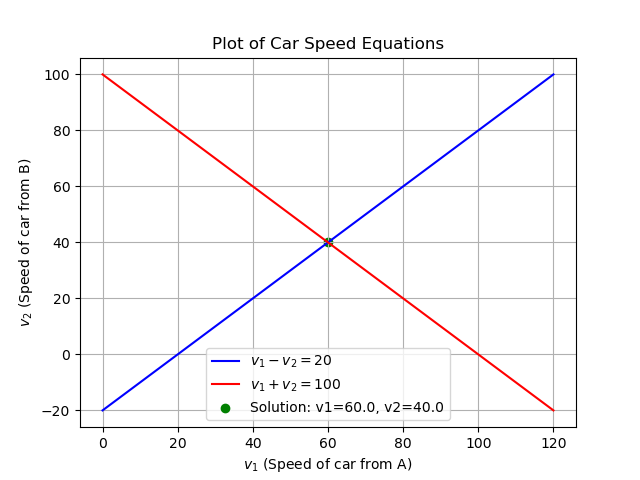
\includegraphics[width=0.7\columnwidth]{figs/Figure_1.png}
    \caption{Graphical Representation of the Solution}
    \label{fig:Plot1}
\end{figure}


\end{document}
